Nền tảng web, cùng với mobile là một trong hai nền tảng chính để phát triển phần mềm phổ biến nhất hiện nay. Để bắt kịp trước sự bùng nổ của nền tảng mobile, nền tảng web cũng thay đổi rất nhiều theo hướng tích cực. Rất nhiều framework, thư viện Frontend mạnh mẽ đã ra đời để giúp lập trình viên xây dựng được những trang web tương tác cao, hiệu suất tốt mà ít tốn công sức, thời gian.
\subsubsection{Single Page Application (SPA)}
Singe Page Application hay Single Page Web Application là một ứng dụng web hay một website mà ở đó tất cả các thao tác của người dùng chỉ diễn ra trên 1 trang duy nhất, tất cả các cấu trúc của trang web (HTML) được load sẵn 1 lần và sẽ không load lại ngay cả khi chuyển trang. Một vài website nổi tiếng như: Gmail, Facebook, Youtube, Twitter,... đều đang sử dụng SPA để tạo nên những trải nghiệm mang tính chiều sâu và chiều rộng cho người dùng.\par
Có rất nhiều nội dung được lặp lại trên đa số các website. Một số thành phần vẫn được giữ nguyên khi người dùng điều hướng trong web (header, footer, logo, navigation bar,...), một số thì chỉ nằm ở những vị trí cố định (filter bar, banner), và còn rất nhiều layout và template được lặp lại (blog, self-service, thiết lập của google mail). SPA sử dụng hiệu quả những sự lặp lại như này và nhờ vào việc linh động viết lại những thành phần cần thay đổi trong trang hiện tại thay vì tải lại toàn bộ 1 trang mới từ sever. SPA loại bỏ sự ngắt quãng khi người dùng đang trải nghiệm những trang nối tiếp nhau, tạo cho người dùng cảm giác như đang sử dụng 1 ứng dụng trên desktop.\par
Sự khác nhau giữa SPA và một web truyền thống (Multiple-page applications): khi người dùng yêu cầu một trang web, thì server sẽ tính toán và trả về trang web đó cho người dùng toàn bộ trang web dưới dạng mã html. Hầu như không có bất kỳ sự liên kết nào giữa 2 yêu cầu gần nhau. Do đó khi có nhiều yêu cầu được diễn ra thì sẽ làm quá trình tính toán diễn ra lâu hơn, bởi hệ thống phải tính toán nhiều thành phần trước khi trả về một trang web hoàn chỉnh. \par
Ưu điểm của SPA:
\begin{itemize}
    \item Load 1 lần cho từng file HTML, CSS, JS.
    \item Hạn chế câu truy vấn đến sever.
    \item Xây dựng Front-end nhanh và có tính tương thích.
    \item Tăng trải nghiệm người dùng.
    \item Giảm thiểu thời gian phát triển và chi phí hạ tầng
\end{itemize}
Nhược điểm của SPA:
\begin{itemize}
    \item Lần load đầu sẽ cực kì nặng.
    \item Đi kèm với sự linh hoạt trong thiết kế SPA thì ta sẽ không có một quy chuẩn nhất định.
\end{itemize}
\subsubsection{Framework ReactJS}
React là thư viện JavaScript phổ biến nhất để xây dựng giao diện người dùng (UI) và có một cộng đồng hỗ trợ đông
đảo. Nó cho tốc độ phản hồi tuyệt vời khi user nhập liệu bằng cách sử dụng phương pháp mới để render trang web. Lập trình viên khi xây dựng SPA bằng React sẽ cảm thấy dễ hiểu mã nguồn mình đang viết, có thể tái sử dụng mã nguồn, tăng tính module hoá cho mã nguồn, giúp việc phát triển một ứng dụng phía người dùng lớn trở nên khả thi. \par
\begin{figure}[h!]
    \begin{center}
        
\includegraphics[width=10cm]{Image/Technical/react_logo.png}
        \caption{ReactJS.}
        \label{reactjs}
    \end{center}
\end{figure}
React nổi tiếng và đi đầu trong cơ chế DOM ảo (Virtual DOM), khi cập nhật một chi tiết trên giao diện, một DOM ảo sẽ được tạo ra, tải lên bộ nhớ, sau đó so sánh với phiên bản DOM ảo trước đó để tìm kiếm sự khác nhau giữa hai phiên bản, từ đó rút ra được những thành phần cần thiết cần cập nhật và giữ nguyên những thành phần còn lại. Điều này là rất tốt về mặt hiệu suất. Mặt khác, cơ chế trên còn giúp mã nguồn dễ hiểu, dễ sửa lỗi hơn. \par
React sửa dụng Encapsulated Components để quản lý trạng thái, sau đó kết hợp chúng lại để tạo ra màn hình giao diện phức tạp. Vì Component được viết bằng JavaScript thay vì HTML template, ta có thể dễ dàng truyền dữ liệu phong phú qua từng thành phần khác nhau, rất linh động và đơn giản. Ngoài ra, React tách hẳn trạng thái của ứng dụng ra khỏi DOM, giúp việc phát triển trở nên dễ dàng vì nhiều thành phần độc lập không ràng buộc với nhau.\par
Ưu điểm của ReactJS:
\begin{itemize}
    \item Dễ sử dụng: React là một thư viện GUI nguồn mở JavaScript tập trung vào một điều cụ thể, hoàn thành nhiệm vụ UI hiệu quả.
    \item Hỗ trợ Reusable Component: React cho phép bạn sử dụng lại components đã được phát triển thành các ứng dụng khác có cùng chức năng. Tính năng tái sử dụng component là một lợi thế khác biệt cho các lập trình viên.
    \item Viết component dễ dàng vì nó sử dụng JSX, mở rộng cú pháp tùy chọn cho JavaScript cho phép bạn kết hợp HTML với JavaScript.
    \item Hiệu suất tốt hơn với Virtual DOM: cho phép xây dựng các virtual DOMs và tổ chức chúng trong bộ nhớ. Nhờ vậy, mỗi khi có sự thay đổi trong DOM thực tế, thì virtual sẽ thay đổi ngay lập tức.
    \item Thân thiện với SEO: React cho phép bạn tạo giao diện người dùng có thể được truy cập trên các công cụ tìm kiếm khác nhau, và có thể tăng tốc quá trình của ứng dụng nên có thể cải thiện kết quả SEO.
\end{itemize}
Nhược điểm của React:
\begin{itemize}
    \item Không có sẵn các tính năng như gọi API, quản lý route, quản lý state,.. cần phải sử dụng thư viện bên ngoài - được phát triển bởi Facebook hoặc
cộng đồng như Redux, React Router, Redux Saga...
    \item React khá nặng nếu so với các framework khác.
    \item Khó tiếp cận cho người mới học Web.
\end{itemize}

\subsubsection{Quản lý router với React Router}
React-Router là một thư viện định tuyến (routing) tiêu chuẩn trong React. Nó giữ cho giao diện của ứng dụng đồng bộ với URL trên trình duyệt. React-Router cho phép bạn định tuyến "luồng dữ liệu" (data flow) trong ứng dụng của bạn một cách rõ ràng. React Router giúp bạn định nghĩa ra các URL động, và lựa chọn Component phù hợp để hiển thị trên trình duyệt người dùng ứng với từng URL.\par
Có ba thành phần chính trong React Router:
\begin{itemize}
    \item Router: BrowserRouter và HashRouter sử dụng History API có trong HTML5 để theo dõi lịch sử bộ định tuyến.
    \item Route matchers: Route và Switch định nghĩa một ánh xạ (mapping) giữa một URL và một Component. Điều đó có nghĩa là khi người dùng truy cập theo một URL trên trình duyệt, một Component tương ứng sẽ được render trên giao diện.
    \item Chuyển hướng: Link, NavLink, và Redirect sử dụng để chuyển qua lại giữa các component.
\end{itemize}

\subsubsection{Quản lý state với kiến trúc Redux}

Một ứng dụng React quản lí state trong các component riêng rẻ, để chia sẻ giữa các component với nhau ta phải truyền từ component cha xuống con hoặc sử dụng đến context và do đó nó chỉ phù hợp với các ứng dụng nhỏ, có ít state. Đối với các ứng dụng lớn có nhiều state thì việc sử dụng context sẽ rất khó phát triển và bảo trì. Redux ra đời giúp cho việc này trở nên đơn giản hơn bằng cách tạo ra Store để lưu trữ toàn bộ data và cùng một nơi và cung cấp nó cho toàn bộ các component trong ứng dụng. (Hình \ref{redux})\par
\begin{figure}[h!]
    \begin{center}
        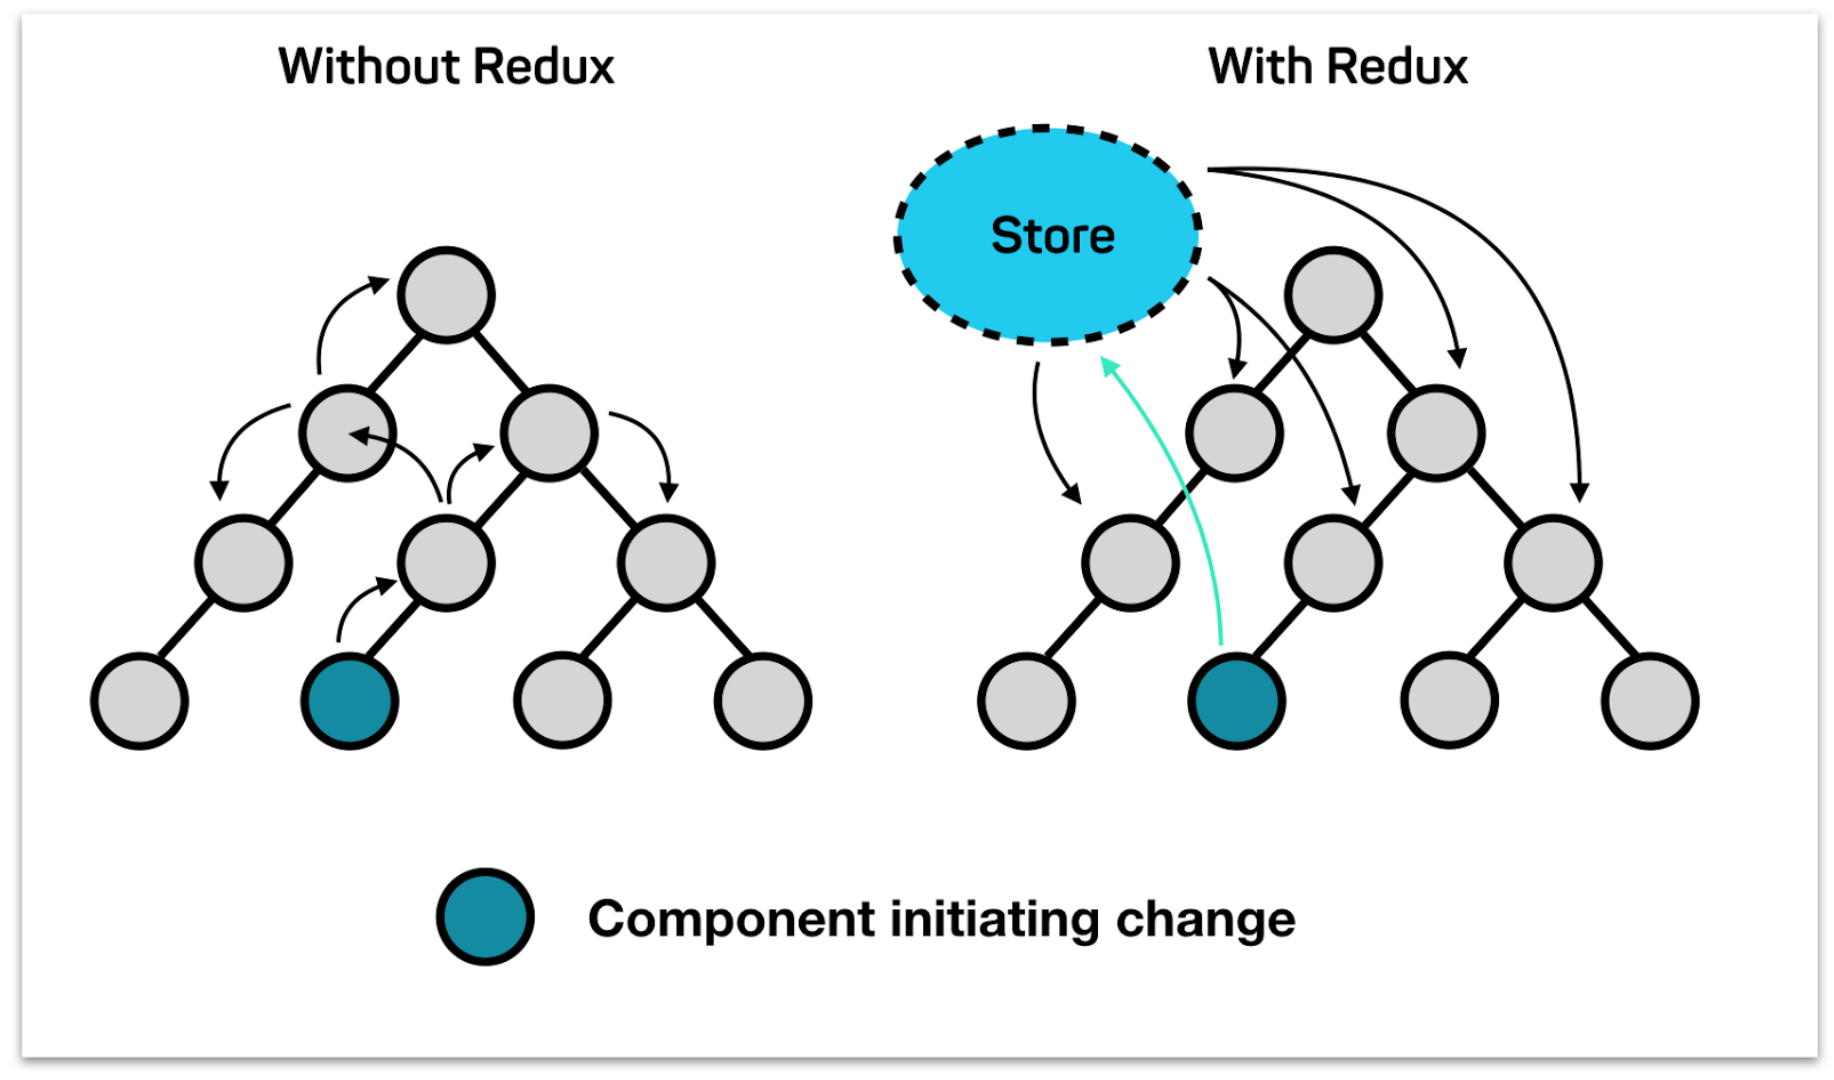
\includegraphics[width=10cm]{Image/Technical/redux.png}
        \caption{Quản lí state với Redux}
        \label{redux}
    \end{center}
\end{figure}
Các thành phần chính của Redux:
\begin{itemize}
    \item Store: là nơi lưu trữ của tất cả state trong ứng dụng, ta có thể truy cập vào để đọc, cập nhật và xóa các state thông qua các actions.
    \item Action: là các sự kiện mà người dùng tạo ra khi tác động vào các view để làm thay đổi state.
    \item Reducer: là một hàm nhận đầu vào là state và các mô tả về sự kiện và dựa vào đó để trả về state mới.
\end{itemize}

Cơ chế hoạt động của Redux (Hình \ref{redux-flow}):
\begin{enumerate}
    \item Ở component xảy ra một sự kiện nào đó của người dùng như nhấn vào một nút, nhấn vào phần tử, tạo hoặc xóa dữ liệu,...
    \item Action nhận được sự kiện trên component và thực hiện tạo một action gồm có kiểu và dữ liệu.
    \item Action này sẽ được gửi đến Reducer thông qua hàm dispatch(action), Reducer sẽ dựa và kiểu của action để lấy các dữ liệu ra tính toán và cập nhật lại dữ liệu của state đó.
    \item Sau khi state này thay đổi, component chứa nó sẽ thực hiện rerender lại.
\end{enumerate}

\begin{figure}[h!]
    \begin{center}
        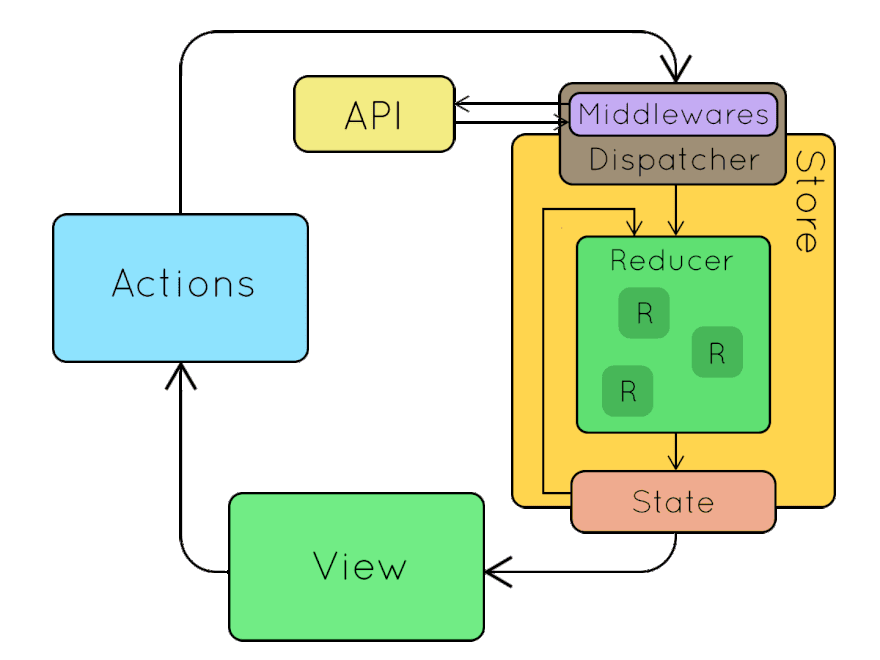
\includegraphics[width=10cm]{Image/Technical/redux-flow.png}
        \caption{Cơ chế hoạt động của Redux}
        \label{redux-flow}
    \end{center}
\end{figure}

\subsubsection{Tích hợp middleware sử dụng Redux Thunk}

Middleware là một lớp nằm giữa Reducer và Dispatch Actions, nó hoạt động sau khi một action được dispatch và trước khi reducer nhận được action này. Middleware trong redux được sử dụng nhiều nhất trong việc xử lí async action - những action không sẵn sàng khi người dùng dispatch, thông thường thì đây là các API request.\par

Hiện nay, có khá nhiều thư viện Middleware cho redux như redux-thunk, redux-saga, redux-observable,... Mỗi thư viện có những phương pháp giải quyết vấn đề riêng, tuy nhiên do thời gian thực hiện luận văn có hạn nên nhóm chọn redux-thunk, thư viện được giới thiệu bởi redux và đơn giản khi hiện thực, làm middleware cho hệ thống của mình.

\subsubsection{Xây dựng ứng dụng với framework Material-UI}

Một ứng dụng ReactJS được xây dựng bằng việc kết hợp các component lại với nhau. Ta có thể xây dựng các component cho ứng dụng bằng cách viết các component sau đó chỉnh sửa CSS từng chút một cho nó. Hiện nay, có khá nhiều thư viện phổ biến cung cấp cho ta các component cơ bản để phát triển giao diện như Boostrap, Material-UI, Ant Design,... Mỗi thư viện trên có các thiết kế theo các chuẩn khác nhau, nhóm đã xem qua và chọn Material-UI vì sự phổ biến, thiết kế đẹp và dễ dàng tùy chỉnh lại các style component một cách dễ dàng.\par
